% Self-contained local starter inspired by the NTNU Laboratory Report in Physics
% template by Vebjorn S. Forde (CC BY 4.0):
% https://www.overleaf.com/latex/templates/ntnu-laboratory-report-in-physics/zrkxstqtpdpv
% This is a simplified adaptation, not the original multi-file project.
% Compile with pdfLaTeX in TeXstudio. Replace the example text and metadata.

\documentclass[5p,a4paper]{elsarticle}

% Common TeX Live packages
\usepackage[utf8]{inputenc}
\usepackage[T1]{fontenc}
\usepackage[english]{babel}
\usepackage{lmodern}
\usepackage{geometry}
\geometry{margin=25mm}
\usepackage{microtype}
\usepackage{graphicx}
\usepackage{amsmath,amssymb}
\usepackage{siunitx}
\usepackage{booktabs}
\usepackage{float}
\usepackage{caption}
\usepackage{enumitem}
\usepackage[hidelinks]{hyperref}
\usepackage[numbers]{natbib}

% ---------- Report details: edit these ----------
\newcommand{\reporttitle}{Uniaxial Tensile Test of Polycarbonate}
\newcommand{\course}{Modern Experimental Mechanics}
\newcommand{\studentname}{Vilmer Dahlberg}
\newcommand{\studentid}{}
\newcommand{\labdate}{2026/11/05}
\newcommand{\submissiondate}{\today}
\newcommand{\institution}{Department of Construction Sciences,  Lund University}

%----------------------------------------------------------
% Math macros
%----------------------------------------------------------
\usepackage{amsmath,amssymb,amsfonts}%
\usepackage{tensor}
\usepackage{upgreek}
\usepackage{sansmath}
\usepackage{xspace}
\usepackage{array}
\usepackage{mathtools}
\newcommand{\bm}[1]{\text{\boldmath{$#1$}}}

\graphicspath{{../results/}, {../figures/}}

\begin{document}
	
	\begin{frontmatter}
	
		\title{\reporttitle}
		\author{\studentname}
		\address{\course\\\institution}
		
		\begin{abstract}
			In this experiment a uniaxial tensile test is performed on a polycarbonate sample. 
		\end{abstract}
		
		\begin{keyword}
			experiment \sep measurement \sep uncertainty
		\end{keyword}
	
	\end{frontmatter}
	
	\section{Introduction}
	Polycarbonate is a type of thermoplastic polymer which, due to its malleability, high strength and toughness, can be found in many modern engineering applications \cite{wikipedia_polycarbonate}. To gain further insight into the material properties of polycarbonate, we perform in this experiment a uniaxial tensile test. The polycarbonate sample, shown in Figure \ref{fig:method:setup}a consists of a thin rectangular brick with two vertically centered circular notches. The sample is mounted in a tensile testing rig, which consists of a) a motor which pulls the sample at a constant rate of displacement (it est displacement controlled loading) and b) a load cell which measures the force required to pull the sample apart. The data is recorded in a LabVIEW \cite{national_instruments_labview_2017} program.
	
	A load cell is used to measure the force. In this experiment the load cell consists of a metal body fitted with a strain gauge. As the load cell deforms due to the external load, the strain gauge deforms, causing a change in electrical resistance. This small difference is measured as a change in voltage and converted into a strain. The stress can then be computed under the assumption of elastic response, which finally gives the force \cite{wikipedia_load_cell}.
	
	Given a cross-section of a continuum body at some spatial point $\bm{x}$ with area $A$ and normal $\bm{n}$ we define the stress vector $\bm{s}$ at that point as
	$$
		\bm{s} = \bm{\sigma}\bm{n} = \lim_{\Delta A \rightarrow 0} \frac{\Delta \bm{P}}{\Delta A}
	$$
	where $\Delta \bm{P}$ the measured traction. Unfortunately, it is in practice impossible to measure the stress directly, for many reasons. Firstly, it's a destructive process, meaning it can realistically only be done once before the sample is destroyed. Secondly, it is impossible to make cross sections with infinitesimally small areas and thirdly any such cross-sections would immediately be out of static equilibrium. Instead we rely on proxies, such as strain, or simplified geometries.
	
	
	Consider a homogeneous cylindrical rod $\mathcal{R}$ with initial length and cross-sectional area $l_0$ and $A_0$. When subjected to a force $P$ along its axial direction the rod will have the new length and cross-sectional areas $l$ and $A$. The (small strain) stretch along its axial direction is given by 
	$$
		\epsilon_E = \frac{l-l_0}{l_0} \implies \frac{V}{V_0} = \left(\epsilon_E + 1\right)\frac{A}{A_0}
	$$
	Furthermore, mechanical equilibrium requires the stress to be equal for any axial-orthogonal cross-section. We are then able to define the \textit{engineering} and \textit{true} stress as
	\begin{align*}
		\sigma_E 	& = \frac{P}{A_0} %
		& \sigma_T	& = \frac{P}{A}
	\end{align*}
	which are related via 
	\begin{equation*}
		\sigma_T = \sigma_E\frac{V}{V_0}\left(\epsilon_E + 1\right)
	\end{equation*}
	
	The goal with this experiment is to perform a tensile test of a polycarbonate sample.
	
	\section{Method}
	Firstly, the sample's dimensions are measured using a caliper. The sample is then loaded into the machine, as shown in Figure \ref{fig:method:setup}b. To ensure that no unintensional torsional forces are applied to the sample, the holding grips are held in place while they are tightened. Once the sample is loaded into the rig its height is measured.
	
	The tensile testing rig is set to displacement controlled loading at a constant rate of $2\,\text{mm}/60\text{s}$. The rig and data acquisition are then simultaneously started. The tensile testing machine is allowed to run until the sample fails, see Figure \ref{fig:method:setup}c, at which point the machine and recording software are stopped.
	
	\begin{figure}
		\centering
		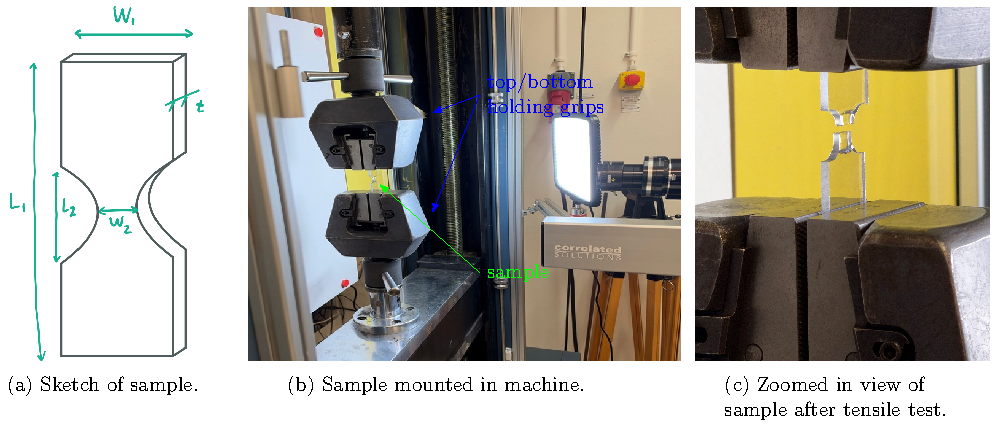
\includegraphics[width=0.5\textwidth]{figure_mosiac.pdf}
		\caption{Mosaic of experimental set-up}
		\label{fig:method:setup}
	\end{figure}
	
	\section{Results and discussion}
	
	\begin{table}
		\caption{Recorded dimensions of polycarbonate sample, in millimeters $[mm]$.}
		\centering
		\begin{tabular}{c|c|c|c|c}
			$L_1$ 	& $L_2$	& $w_1$	& $w_2$ & $t$ 	\\
			\hline
			80.6	& 10.0	& 25.5	& 9.7 	& 3.1 	\\
		\end{tabular}
		\label{tab:method:polycarbonate dimensions.}
	\end{table}
	
	The recorded lengths are shown in Table \ref{tab:method:polycarbonate dimensions.} and the acquired force-displacement data is shown in Figure \ref{fig:force_displacement}. To take into account calibration errors, the final force was scaled by $26.07$. The data was calibrated such that the load at the final time step is zero, which is consistent with the fact that the sample has failed. This implies that the sample was under some tension from the beginning due to fastening it too tight in the rig. The maximum load and load at failure is $1.87\,\text{kN}$ and $1.60\,\text{kN}$ respectively corresponding to engineering stresses of $62.05\,\text{MPa}$ and $53.16\,\text{MPa}$, respectively. 
	
	The first thing to note is that the gathered force data is a reflection of the samples macroscopic response to the applied load. As such, it is hard to draw any meaningful conclusions about the material behavior, i.e. the local response. To do any such analysis we require stress and strain measurements. Furthermore, it is worth noting that the data comes from one single sample. The experiment should ideally be repeated multiple times to take into account measurement errors, the human factor and so on. Finally, it is noted that the sample is heterogeneous, but treated as homogeneous.
	
	Initially, the force does not increase linearly with the applied displacement, which suggests that the material is either undergoing hyper-elastic or plastic deformations. Unfortunately, it is impossible to distinguish these behaviors without unloading the sample. Once the force reached its peak value, it quickly decreased, suggesting some sort of stress redistribution. Notably, are able to capture this behavior, due to using displacement controlled loading. Finally, the force increased until the sample failed. Simultaneously, the sample's thickness decreased significantly. As such, it's hard to know if the stress actually increased, which would otherwise suggest hardening, decreased (suggesting softening) or even remained constant.
	
	
	\begin{figure}[t]
		\centering
		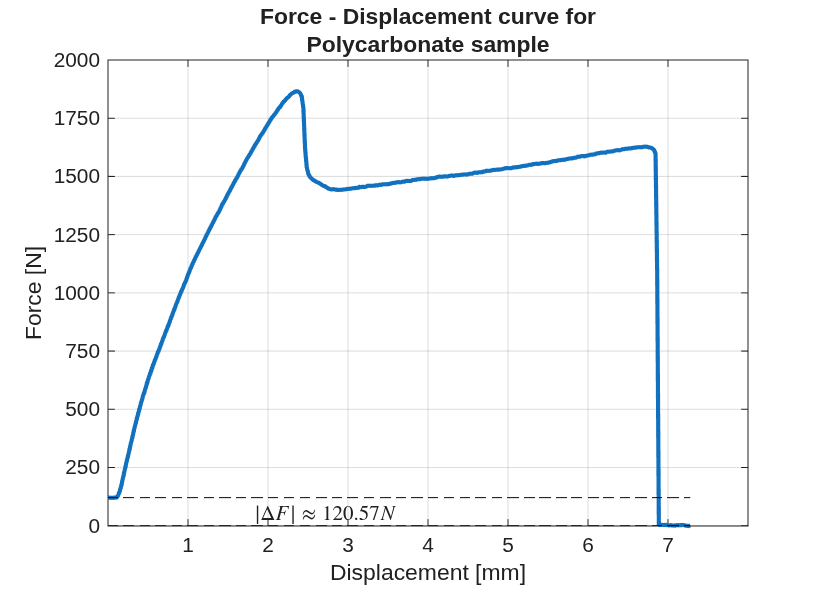
\includegraphics[width=0.5\textwidth]{force_displacement.png}
		\caption{Plot of the force-time data gathered during the tensile test. The force-displacement graph can be inferred from the displacement rate by scalar multiplication.}
		\label{fig:force_displacement}
	\end{figure}
	
	
	\section{Conclusions}
	In this experiment a uniaxial tensile test was successfully performed on a polycarbonate sample. Not much can be said about the material behavour from the force-displacement data.
	
	\bibliographystyle{unsrtnat}
	\bibliography{refs.bib}
	
\end{document}
